\chapter{Building Blocks of WSN} \label{Chp: Building Blocks}

%In this chapter, we will start by introducing the building components of WSN, mainly focuses on different protocol options at each layer. Then we move to security related work, in three aspects of traffic analysis attacks against different Internet applications, attacks against certain protocols and methods for detecting information leakage in different scenarios. Finally we conclude the chapter by cross referencing those  attacks on Internet to the observable metadata in WSN, proposing the potential traffic features that may lead to information leakage.
In this chapter, we introduce the building blocks of a WSN by OSI model\cite{OSI}.

In OSI model, the data channel is constructed layer by layer from the physical medium at the bottom to the abstracted application at the top (\Cref{fig: OSI model}). Each layer serves a specific purpose, from how to transmit a bit between two physically connected devices to how applications interprets the data. by introducing different protocol options at each layer.

Before the application data is being sent over the wire, two ends of the communication must agree on protocols being used at each layer. The data is then encapsulated from top layer down to the bottom, as depicted in \Cref{fig: OSI channel}. Each encapsulation adds additional metadata, namely protocol headers, to the data. The process is unwound at the receiving side. Normally lower layer protocols are transparent to upper layers.The outputted encapsulated data from upper layer is simply treated as the payload to a lower layer protocol.

In many cases the boundaries between top three layers are ambiguous; thus they are all referred as Application Layer for convenience.
\begin{figure*}
	\centering
	{
		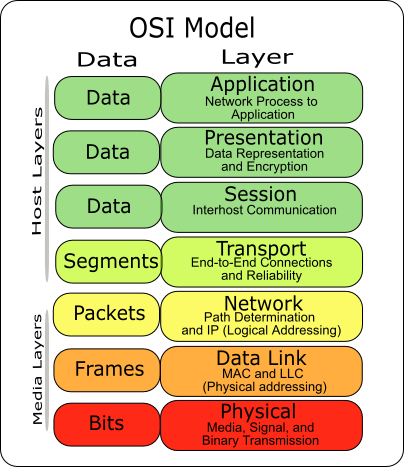
\includegraphics[width=0.4\textwidth,]{fig/Osi-model-jb.png}
	}
	\caption{OSI model} \label{fig: OSI model}
\end{figure*}

\begin{figure*}
	\centering
	{
		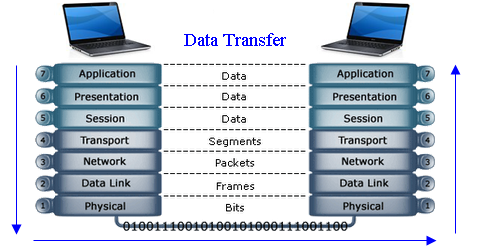
\includegraphics[width=0.6\textwidth,]{fig/osi-model.png}
	}
	\caption{Data Transfer in OSI model} \label{fig: OSI channel}
\end{figure*}

In network terminology, 8 bits is called an OCTET. For the purpose of readability we use the general computer science term BYTE to represent the unit consists of 8 bits.

A combination of protocols at each layer is called a protocol stack, or a protocol suite. The protocol stack until application layer are usually handled by the operating systems. There are several systems specifically aimed to support WSN applications. Contiki\cite{Contiki} is a highly customisable system with 6LoWPAN protocol stack with many hardware supported, OpenWSN\cite{OpenWSN} also has a well hardware support and is featuring full protocol support up to CoAP\cite{rfc7252}, FreeRTOS\cite{FreeRTOS} is optimised for real time tasks, etc.

Due to popularity, in this report we mainly focus on Contiki and the 6LoWPAN protocol stack.

\section{Physical Layer}
Physical Layer specifies the hardware requirements for devices. It defines data transmission at bit level.

WSN features, as explained by its name, wireless connectivity. 802.15.4\cite{802154} standard is supported in many recent WSN devices. Its Physical Layer specification is intended to be for embedded devices emphasising low energy, low cost and low speed. Bluetooth Low Energy, BLE, is another candidate for WSN with similar features. \cite{802154BLE} provides a performance analysis of 802.15.4 and BLE.

Usually the length MAC frame, which we explain in \Cref{Sec: Data Link Layer}, is announced before it is being transmitted, e.g. shown in \Cref{Fig: 802.15.4 PHY Frame}.

\begin{table}[h!]
	\centering
	\begin{tabular}{|l|l|l|l|}
		\hline
		Preamble & SFD & MAC frame Length & Reserved \\ \hline
	\end{tabular}
	\caption{802.15.4 PHY Frame}
	\label{Fig: 802.15.4 PHY Frame}
\end{table}

Preamble is used for hardware synchronisation. Start Frame Delimiter is a constantly 0xE5 for 802.15.4 frames. The length of a MAC frame is 0 to 127 bytes. More details can be found in \cite{802154}.

\section{Data Link Layer} \label{Sec: Data Link Layer}
Data Link Layer solves the problem of how the media is controlled. It also defines the atomic data chunk, called frames, being transmitted over the physical channel. Data Link protocols are strongly related to physical features of underlining devices. This layer is sometimes referred as MAC layer and the frame is called MAC frame in many context. MAC protocol only solves single hop communication. Packet forward is defined in upper layer protocols.

With respect to Media Access Control, MAC, technologies such as CSMA/CA \cite{802154} standard and TSCH\cite{TSCH} provides solutions to at which timing and channel should the radio transceiver send and receive data. ContikiMAC\cite{ContikiMAC} proposes a Radio Duty Cycle, RDC, protocol that aims to be energy efficient and has been implemented on Contiki OS.

Another major component in Data Link Layer protocols is the format of different types of frames. In this research, we focus on 802.15.4 standard as its increasing attention in both industry and academy. 

Implementing security measures at this layer is called Link Layer SECurity, LLSEC. 

\subsection{802.15.4 MAC Layer}

There are four types of frames defined in this standard, which are:
\begin{description}
	\item[\textbf{Beacon}] broadcastes to physically organise the network.
	\item[\textbf{Command}] is used in network maintenance.
	\item[\textbf{Data}] carries actual payload.
	\item[\textbf{ACK}] only optionally sent in response when requested.
\end{description}

Among these types of frames, we are particularly interested in Data frames. We will explain our concern of this choice later in \Cref{Sec: Leakage Sources}. \Cref{Fig: 802154 frame} describes the format of a 802.15.4 Data frame.

\begin{figure*}[h!]
	\centering
	\begin{tabular}{|c|c|c|c|c|}
		\hline
		\multicolumn{3}{|c|}{MAC Header}                           & MAC Payload & MAC Footer     \\ \hline
		2 (bytes)     & 1                    & 4 to 20              & *           & 2              \\ \hline
		Frame Control & Data Sequence Number & Address Information & Data        & Frame Checksum \\ \hline
	\end{tabular}
	\caption{802.15.4 Data Frame}
	\label{Fig: 802154 frame}
\end{figure*}

We briefly explain the format of 802.15.4 Data frame.
\begin{description}[style=nextline]
	\item[\textbf{Frame Control}]
	This 2 bytes field contains the bit flags of additional information that instructs how the receiver should interpret this frame, including the type of this frame, whether the security option is enabled and how the source and destination addresses are represented. When the security option is enabled, additional field will be added to the frame. We will explain the security enabled frame format later in \Cref{Sec: Data Link Layer}. A full explanation of the flags can be found in \cite{802154}.
	
	\item[\textbf{Sequence Number}]
	Each packet is assigned a sequence number. The main purpose of this field is that it enables a simple acknowledgement mechanism, ACK, at MAC layer. Since MAC layer provides only unreliable transmission, i.e. MAC frames are allowed to be dropped or arrive disordered; hence the ACK is optional. However, some other protocol can utilise this ACK, e.g. ContikiMAC uses the ACK MAC frame to inform the sender that the frame is received and hence terminates the resending process of sender.
	
	\item[\textbf{Address Information}]
	This field contains the source address and destination address of this frame. The length of address is variable. Simply speaking, a longer addresses is used for larger network. and shorter for smaller. Each device has a unique built in address as known as MAC address. The MAC address is configurable on some, in fact nearly all recently, devices. Broadcast is achieved by using a specific destination address but group multicast is not implemented on this layer. In fact, given the physical character of radio, both broadcast messages and unicast messages are technically broadcasted. It entirely depends on the receiver to dropping frames that specifies an unicast address of other nodes.
	
	\item[\textbf{Data}]
	This is the MAC layer data. This data is constituted of upper layer protocol headers and application data.
	
	\item[\textbf{Frame Checksum}]
	The checksum is used to check and correct the error induced by physical channel.
\end{description}

The Frame Control, Sequence Number and Address Information together are called MAC header. The Data field is called MAC payload accordingly. 

802.15.4 standard specifies the Maximum Transmission Unit, MTU, to be 127 bytes including the MAC header and footer. That is to say any 802.15.4 compatible hardware must be able to send at least 127 bytes within one frame; any frame that is larger than this size is not guaranteed to be support by the device. Since the MAC header and footer consumes 25 bytes in a Data frame, there is actually 102 bytes left for MAC payload.

Setting the security flag in Frame Control enables 802.15.4 security and adds additional information into the MAC header. We introduce the 802.15.4 security later in \Cref{Subsec: 802154 Sec}.

\subsection{802.15.4 Security} \label{Subsec: 802154 Sec}
802.15.4 security is based on symmetric cryptography, namely Authenticated Encryption with Associated Data, AEAD, scheme. To be more specifically, it provides encryption for MAC payload and authenticity for both MAC header and payload. The cryptographic primitive adopts AES-128 as the block cipher.

802.15.4 has a set of configurable security levels:
\begin{itemize}
\item Encryption only, i.e. only MAC payload is encrypted in CTR mode.
\item Authentication only, i.e. a tag is attached at the end of Data field. The tag is computed on MAC header and MAC payload in CBC mode. The MAC payload is transmitted in plaintext.
\item Encryption and authentication. The whole frame is processed in CCM*\cite{802154} mode, with MAC header being the associated data and MAC payload being the plaintext to be encrypted. The asterisk symbol represents a slight restriction which requires the nonce, or IV, must contain the encoded format specifier that can uniquely determine the format of output ciphertext. In other words, the receiver must can uniquely determine solely by nonce whether authentication and encryption are enabled as well as the length of authentication tag.
\item The tag can be further configured to be 32 bit, 64 bit or 128 bit when authentication is enabled.
\end{itemize}

The format of a 802.15.4 Data frame with security option set is described in \Cref{Fig: 802154 sec frame}.

\begin{figure*}[h!]
	\centering
	\begin{tabular}{|c|c|c|c|c|c|c|}
		\hline
		\multicolumn{4}{|c|}{MAC Header}                                                             & \multicolumn{2}{c|}{MAC Payload} & MAC Footer     \\ \hline
		\multicolumn{3}{|c|}{\multirow{2}{*}{As MAC header in \Cref{Fig: 802154 frame}}} & 0 to 14                    & *             & 0/4/8/16         & 2              \\ \cline{4-7} 
		\multicolumn{3}{|c|}{}                                           & Auxiliary Security Header & Data          & MIC              & Frame Checksum \\ \hline
	\end{tabular}
	\caption{802.15.4 Frame with security option enabled} \label{Fig: 802154 sec frame}
\end{figure*}

The Auxiliary Security Header contains the additional information needed by 802.15.4 security.

\begin{description}[style=nextline]
	\item[\textbf{Security Level}]
	Security Level is represented by the first 3 bits in Auxiliary Security Header. The highest bit controls whether encryption is enabled. The lower two bits controls the length of MIC with the value $0$ indicates no authentication.
	\item[\textbf{Frame Counter}]
	This 4 byte filed increases by one for each frame sent. It is also used for replay detection.
	\item[\textbf{Key Strategy}]
	The other parts instructs which key to be used for this frame. The keys are presumed to be pre-shared in PAN Information Base, PIB, which is a database containing information that is shared among the network. Keys are managed by groups and indexes within a group. The definition of groups depends on upper layer applications.
\end{description}

More details of Auxiliary Security Header is defined in the 802.15.4 standard.

Message Integrity Code, MIC, is equivalent to the cryptography term Message Authenticate Code, MAC. Therefore the term MIC is used to avoid confusion with Media Access Control.

Access Control List, ACL, is a list data structure defined in 802.15.4. It is used to maintain 802.15.4 security access during runtime.Each entry in ACL is paired with another node.  An ACL entry contains the following elements:
\begin{description}
	\item[\textbf{Address}] The address of remote node, used as an identifier.
	\item[\textbf{Security Suite}] The security level to use associated to the address.
	\item[\textbf{Key}] The paired cryptographic key associated to the address.
	\item[\textbf{Last Initial Vector}] Nonce used for the last outgoing frame.
	\item[\textbf{Replay Counter}] Nonce received for the last incoming frame.
\end{description}
On sending a frame with security option, the sender looks up destination address in ACL and determines the security level, key and frame counter which is encoded into the last initial vector. On receiving a frame, the receiver looks up source address in ACL and checks for match of the security suite and security level in the frame. Then it verifies the frame with the key. If replay protection is enabled, the replay counter is also compared. Failing any of the tests will result into rejecting of the frame.

\subsection{Nonce of CCM* in 802.15.4 security}
As stated earlier in \Cref{Subsec: 802154 Sec}, CCM* requires that the format of ciphertext can be uniquely deduced from the nonce. \Cref{Fig: CCM nonce} describes the nonce used for encryption.

\begin{figure*}[h!]
	\centering
	\begin{tabular}{|c|c|c|c|c|}
		\hline
		1 (bytes) & 8              & 4             & 1              & 2             \\ \hline
		Flag      & Source Address & Frame Counter & Security Level & Block Counter \\ \hline
	\end{tabular}
	\caption{CCM* nonce for encryption}
	\label{Fig: CCM nonce}
\end{figure*}

\begin{description}
\item[\textbf{Flag}]
This is a constant a value equals to 0x02.
\item[\textbf{Source Address}]
This field is the address of sender. If an address of length than 8 byte is used, it will be extended to 8 byte.
\item[\textbf{Frame Counter}]
The frame counter is directly mapped from the same filed in Auxiliary Security Header, as described earlier.
\item[\textbf{Security Level}]
As of frame counter, security level is also directly mapped from Auxiliary Security Header with the highest bit set to $0$. As described earlier, security level solely determines the format of ciphertext.
\item[\textbf{Block Counter}]
This is exactly the block index of MAC payload, increases by one for each block. Since AES-128 is the underlining block cipher; therefore the block size is 128 bit.
\end{description}

802.15.4 security could either be implemented by hardware and/or software. Some platform may not support the security option, or only supports a sub set of this measure. We briefly describe an implementation on Contiki platform later in \Cref{Subsec: noncoresec}.

\subsection{Implementation on Contiki: noncoresec} \label{Subsec: noncoresec}
noncoresec is the LLSEC implementation on Contiki. It is a reduced implementation of 802.15.4 security which supports only a network shared key hard coded into the kernel code.

\section{Network Layer}
The Data Link Layer protocol has solved the problem of data transmission over directly linked nodes. However, real world WSN applications are sometimes deployed in a wider range that not all nodes can be directly connected, such as a smart city application. The solution to build a logic data path between the nodes where each intermediate node forwards the data to the next node until it reaches its destination. Such logical data path is called a multi hop connection and directly connected data path is called a single hop connection respectively. The transmission unit at the Network Layer is called a packet.

A network is defined as a set of nodes logically connected to each other. There are two common types of network considered in WSN applications:
\begin{description}[style=nextline]
	\item[\textbf{Star Network}]
	Star network is a centralised network, as in \Cref{fig: Star Network}. Each node is directly linked to the centre. Star networks can be easily implemented and thus requires less resources.
	\item[\textbf{Mesh Network}]
	Mesh network has a decentralised structure as shown in \Cref{fig: Mesh Network}. Every node is capable to forward packets. Comparing to star network, mesh network is more flexible and scalable but also more complicate and harder to implement. Mesh network is more practical than star network in large scale applications, such as smart cities.
\end{description}

\begin{figure*}
	\centering
	\begin{subfigure}[b]{0.5\textwidth}
		{
			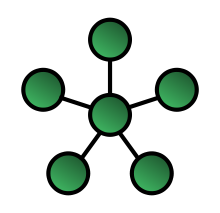
\includegraphics[width=0.5\textwidth,]{fig/StarNetwork.png}
		}
		\subcaption{Star Network} \label{fig: Star Network}
	\end{subfigure}
	\begin{subfigure}[b]{0.5\textwidth}
		{
			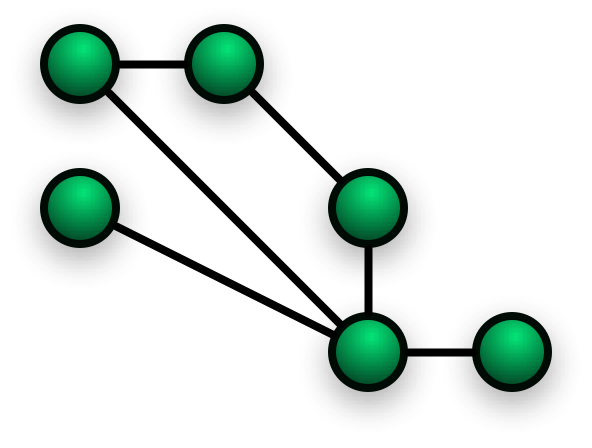
\includegraphics[width=0.5\textwidth,]{fig/NetworkTopology-Mesh.png}
		}
		\subcaption{Mesh Network} \label{fig: Mesh Network}
	\end{subfigure}
	\caption{Network Topologies} \label{fig: Network topologies}
\end{figure*}

Some network are built with a hybrid approach of star network and mesh network, e.g. the Cluster Tree Network of Zigbee\cite{zigbee} as showed in \Cref{fig: ZigBee Topologies}.

\begin{figure*}[h!]
	\centering
	{
		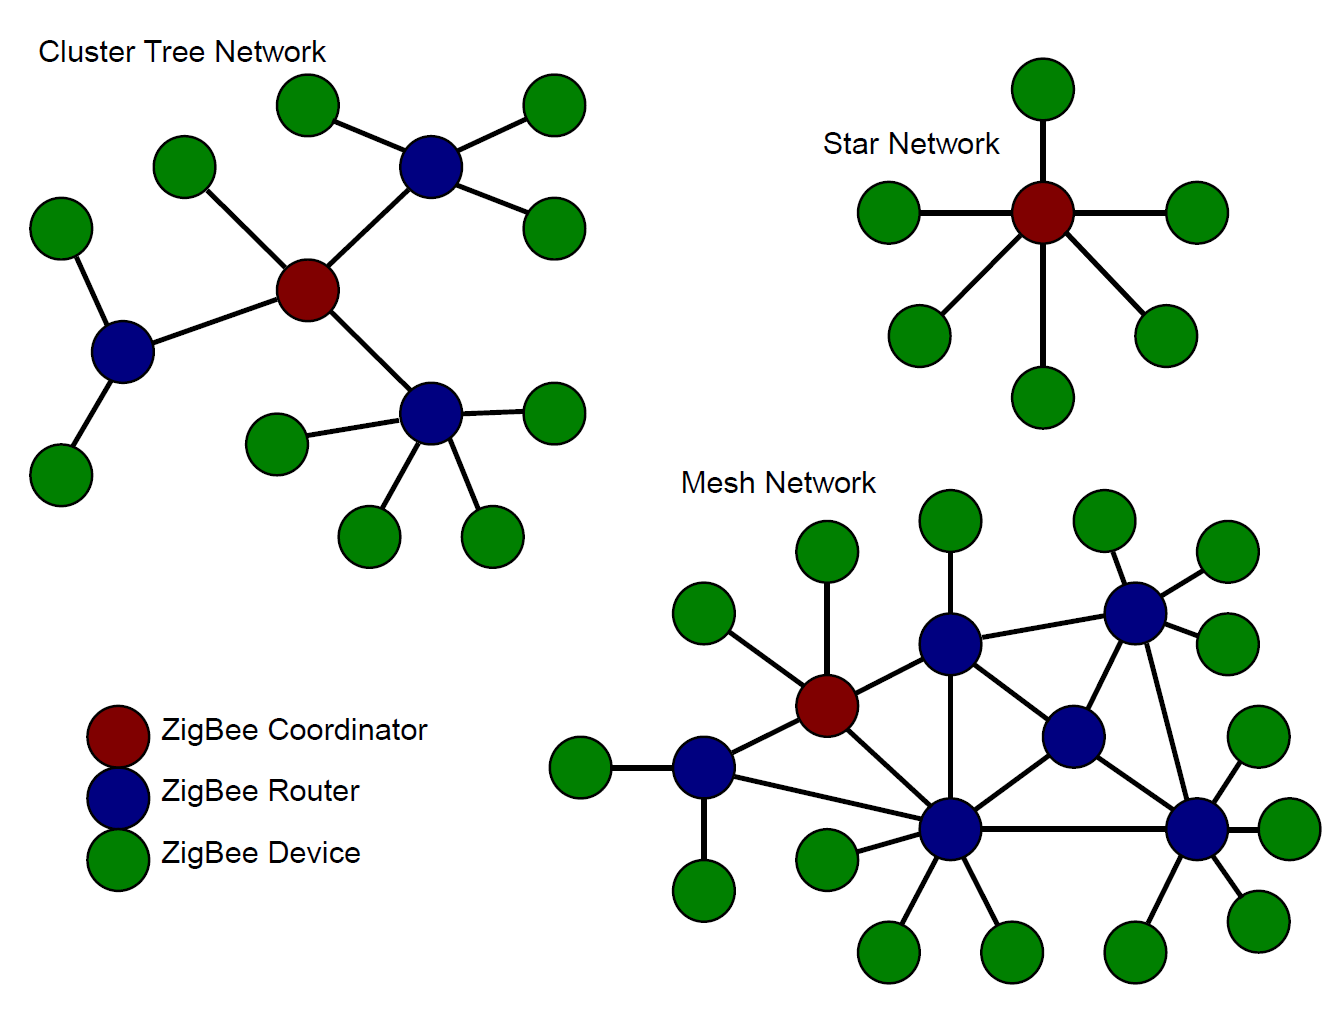
\includegraphics[width=0.7\textwidth,]{fig/ZigBeeTopologies.png}
	}
	\caption{Different ZigBee Network Topologies} \label{fig: ZigBee Topologies}
\end{figure*}

In this report we are particularly interested into the emerging WSN standard 6LoWPAN. 6LoWPAN is an IPv6 based mesh network that is specifically designed to fit into low power wireless devices. 6LoWPAN has the following features making it popular in IoT industry: 
\begin{itemize}
	\item Each device is assigned with an IPv6 address of compressed format. With a border router that translates the compressed IPv6 address into an IP address, a node inside 6LoWPAN  can directly communicate with a host over Internet.
	\item Its mesh routing feature lead to a flexible, scalable and robust network, as the network can spontaneously reorganise itself at running time.
	\item It is standardised by IETF and well supported in industry.
\end{itemize}

As of this project, we are specifically interested into the packets generated in a 6LoWPAN network. A sub layer is defined in 6LoWPAN standard\cite{rfc4944} to compress a standard IPv6 header, in order to reduce the overhead induced by protocol stacks and provide more bandwidth to the applications. Additional headers are prepended before the IPv6 header as shown in \Cref{Fig: IPv6 Header Compression}. 

\begin{figure*}[h!]
	\centering
	\begin{tabular}{|l|l|l|}
		\hline
		Header Compress Information & Compressed IPv6 Header & IPv6 Payload \\ \hline
	\end{tabular}
	\caption{IPv6 Header Compression}
\label{Fig: IPv6 Header Compression}
\end{figure*}

Simply speaking, the compression is done by following methods:
\begin{itemize}
\item Optimised encoding. Take the Hop Limit, HLIM or TTL (Time To Live), field for example, the frequently used values, which are 1, 64 and 255, are represented in 2 bits as 01b, 10b and 11b respectively. 
\item Use a reduced sub set of values of certain fields in a standard IPv6 header.
\end{itemize}

Generally speaking, packets in a 6LoWPAN can be categorised into two classes:
\begin{enumerate}
	\item \textbf{Header Compressed IPv6 Packet}
	\item \textbf{ICMPv6 Packet}
\end{enumerate}

We give a brief explanation of their contents in \Cref{Compressed IPv6} and \Cref{ICMPv6} respectively.

\subsection{Header Compressed IPv6 Packets} \label{Compressed IPv6}

\subsection{ICMPv6 Packets} \label{ICMPv6}

\section{Transport Layer}

\section{Application Layer}

\section{Other protocols and standards}
